\documentclass[11pt]{article}

\usepackage[margin=1.0in]{geometry}
\usepackage{enumitem}
\usepackage{tabularx}
\usepackage{pdfpages}
\usepackage{hyperref}
\hypersetup{
    colorlinks=true,
    linkcolor=blue,      
    urlcolor=cyan,
}

\urlstyle{same}

\newcommand{\code}[1]{\texttt{#1}}
\newcolumntype{L}[1]{>{\raggedright\arraybackslash}p{#1}}
\newcolumntype{C}[1]{>{\centering\arraybackslash}p{#1}}
\newcolumntype{R}[1]{>{\raggedleft\arraybackslash}p{#1}}

\begin{document}

\title{\textbf{Expression Calculator} \\
    \url{https://github.com/stepheniskander/csc380project}}
\author{Nicholas Esposito \\ nesposi3@oswego.edu \and Stephen Iskander \\ siskande@oswego.edu}

\maketitle

\section{Project Description}
Our project is an expression calculator.
The user can input mathematical expressions (e.g. \code{4*2+1}) to be evaluated to a numerical answer.
Expressions can also contain matrices or calculus operations such as integrals and derivatives.


\par The program uses JavaFX for its user interface.
The main window is a simple command-prompt-like interface that the user types expressions or equations into.
Expressions are typed into a text field at the bottom of the window, and the expression as well as its evaluated answer are displayed in a text area above the input field.
The user can see their history in the output area so they can easily copy and paste previous expressions.



\newpage

\section{System Requirements}

\begin{center}
\begin{tabular}{|L{.5in}|R{.5in}|L{5in}|}
\hline
\multicolumn{1}{|c|}{\textbf{Identifier}} & \multicolumn{1}{c|}{\textbf{Priority}} & \multicolumn{1}{c|}{\textbf{Description}} \\ \hline
REQ1  & 10 & Parsing user input into an expression. \\ \hline
REQ2  & 10 & Provide an interface for user to input expressions and see result.\\ \hline
REQ3  & 10 & Evaluate expression parse tree into numerical answer. \\ \hline
REQ4  & 8  & Evaluate calculus operations numerically. \\ \hline
REQ5  & 7  & Evaluate calculus operations symbolically. \\ \hline 
REQ6  & 7  & Parse a matrix entered in text format ([[x y z] [a b c]]) \\ \hline
REQ7 & 7 & Calculate matrix multiplication of two matrices \\ \hline

\end{tabular}
\end{center}

\newpage

\section{User Stories}

\begin{center}
\begin{tabular}{|L{.5in}|R{.5in}|L{5in}|}
\hline
\multicolumn{1}{|c|}{\textbf{Identifier}} & \multicolumn{1}{c|}{\textbf{Size}} & \multicolumn{1}{c|}{\textbf{Description}} \\ \hline
ST-1 & 3 pts & As a user, I can evaluate an expression by typing in the input field. \\ \hline
ST-2 & 4 pts & As a user, I can evaluate an expression containing calculus operations numerically. \\ \hline
ST-3 & 4 pts & As a user, I can input a matrix in a text format. \\ \hline
ST-4 & 5 pts & As a user, I can perform matrix multiplication. \\ \hline
\end{tabular}    
\end{center}

\newpage

\section{Use Cases}

\begin{center}
\begin{tabular}{p{1.5in}p{5in}}
\hline
\textbf{Use Case UC-1}     & \textbf{EvaluateExpression} \\ \hline
Related Requirements: & REQ1, REQ2, REQ3 \\
Initiating Actor:     & User \\
Participating Actors: & GUI, ExpressionParser, Expression \\
Actor's Goal:          & To evaluate a mathematical expression typed into the calculator. \\
Preconditions:         & \begin{itemize}[nosep]
                         \item GUI is visible
                         \item ExpressionParser is initialized
                         \end{itemize} \\
Postconditions:        & \begin{itemize}[nosep]
                         \item Program is ready to evaluate another expression.
                         \end{itemize} \\ \hline
\end{tabular}

\begin{tabular}{p{.25in}p{.25in}p{5.8in}}
\multicolumn{3}{l}{Flow of Events for Main Success Scenario:} \\
$\rightarrow$ & 1. & The User types an expression into the input field and presses enter. \\
            & 2. & \code{include::ParseExpression} \\ 
$\leftarrow$  & 3. & Expression object evaluates to a number \\
$\leftarrow$  & 4. & GUI displays answer to User \\
\end{tabular}

\begin{tabular}{p{.25in}p{.25in}p{5.8in}}
\multicolumn{3}{l}{Flow of Events for Extensions:} \\
\multicolumn{2}{c}{\textbf{3a.}} & User entered an expression that cannot be evaluated \\
$\leftarrow$  & 1.           & Expression throws ArithmeticException
\end{tabular}
\end{center}



\newpage

\begin{center}
\begin{tabular}{p{1.5in}p{5in}}
\hline
\textbf{Use Case UC-2}     & \textbf{ParseExpression} \\ \hline
Related Requirements: & REQ1 \\
Initiating Actor:     & GUI \\
Participating Actors: & ExpressionParser, Expression \\
Actor's Goal:          & To parse the incoming string into an evaluable expression. \\
Preconditions:         & \begin{itemize}[nosep]
		      \item  ExpressionParser is initialized
                         \end{itemize} \\
Postconditions:        & \begin{itemize}[nosep]
                         \item An Expression object is created and ready to be evaluated.
                         \end{itemize} \\ \hline
\end{tabular}

\begin{tabular}{p{.25in}p{.25in}p{5.8in}}
\multicolumn{3}{l}{Flow of Events for Main Success Scenario:} \\
$\rightarrow$ & 1. & String with Expression information comes from the GUI. \\
$\leftarrow$  & 2. & Diykstra's Shunting Yard Algorithm is used to convert the input in normal notation into Reverse Polish Notation\\
$\leftarrow$  & 3. & An Expression object is created that stores the  RPN in a Stack \\
\end{tabular}

\begin{tabular}{p{.25in}p{.25in}p{5.8in}}
\multicolumn{3}{l}{Flow of Events for Extensions:} \\
\multicolumn{2}{c}{\textbf{2a.}} & User entered an expression with invalid characters \\
$\leftarrow$  & 1.           & ExpressionParser throws NoSuchElementException\\

\multicolumn{2}{c}{\textbf{2b.}} & User entered an equation\\
 & 1.           & \code{extend::ParseEquation}\\

\end{tabular}
\end{center}



\newpage
\begin{center}
\begin{tabular}{p{1.5in}p{5in}}
\hline
\textbf{Use Case UC-3}     & \textbf{Integrate} \\ \hline
Related Requirements: & REQ4, REQ5 \\
Initiating Actor:     & User \\
Participating Actors: & GUI, Polynomial \\
Actor's Goal:          & To integrate an expression symbolically or definitively. \\
Preconditions:         & \begin{itemize}[nosep]
		      \item  Polynomial is initialized
                         \end{itemize} \\
Postconditions:        & \begin{itemize}[nosep]
                         \item An indefinite integral is calculated, or a definite integral if given range parameters.
                         \end{itemize} \\ \hline
\end{tabular}

\begin{tabular}{p{.25in}p{.25in}p{5.8in}}
\multicolumn{3}{l}{Flow of Events for Main Success Scenario:} \\
$\rightarrow$ & 1. & User inputs a fucntion to integrate.\\
$\leftarrow$  & 2. & A Polynomial object is parsed from User input.\\
$\leftarrow$  & 3. & An indefinite integral is calculated from the function.\\
$\leftarrow$  & 4. & If given range parameters, the application displays a numerical answer. Otherwise, it returns an indefinite integral function. 
\end{tabular}

\begin{tabular}{p{.25in}p{.25in}p{5.8in}}
\multicolumn{3}{l}{Flow of Events for Extensions:} \\
\multicolumn{2}{c}{\textbf{2a.}} & User entered an invalid function \\
$\leftarrow$  & 1.           & Polynomial throws Exception.\\
\end{tabular}
\end{center}



\newpage

\begin{center}
\begin{tabular}{p{1.5in}p{5in}}
\hline
\textbf{Use Case UC-4}     & \textbf{Derive} \\ \hline
Related Requirements: & REQ4, REQ5 \\
Initiating Actor:     & User \\
Participating Actors: & GUI, Polynomial \\
Actor's Goal:          & To derive the expression symbollically or at a point. \\
Preconditions:         & \begin{itemize}[nosep]
		      \item  Polynomial is initialized
                         \end{itemize} \\
Postconditions:        & \begin{itemize}[nosep]
                         \item A derivative function is calculated, and optionally evaluated at a single point.
                         \end{itemize} \\ \hline
\end{tabular}

\begin{tabular}{p{.25in}p{.25in}p{5.8in}}
\multicolumn{3}{l}{Flow of Events for Main Success Scenario:} \\
$\rightarrow$ & 1. & The user inputs a function.\\
$\leftarrow$   & 2. & A Polynomial object is parsed from the input.\\
$\leftarrow$   & 3. & A derivative function in generated from the parsed function.\\
$\leftarrow$   & 4. & Either the generated derivative function or the derivative at a certain point is displayed to the user.\\ 
\end{tabular}

\begin{tabular}{p{.25in}p{.25in}p{5.8in}}
\multicolumn{3}{l}{Flow of Events for Extensions:} \\
\multicolumn{2}{c}{\textbf{2a.}} & User entered an invalid function \\
$\leftarrow$  & 1.           & Polynomial throws Exception.\\
\end{tabular}
\end{center}

\newpage
\begin{center}
\begin{tabular}{p{1.5in}p{5in}}
\hline
\textbf{Use Case UC-5}     & \textbf{ParseMatrix} \\ \hline
Related Requirements: & REQ6 \\
Initiating Actor:     & GUI \\
Participating Actors: &MatrixParser, Matrix \\
Actor's Goal:          & To parse the incoming string into a Matrix. \\
Preconditions:         & \begin{itemize}[nosep]
		      \item  MatrixParser is initialized
                         \end{itemize} \\
Postconditions:        & \begin{itemize}[nosep]
                         \item A Matrix object is created.
                         \end{itemize} \\ \hline
\end{tabular}

\begin{tabular}{p{.25in}p{.25in}p{5.8in}}
\multicolumn{3}{l}{Flow of Events for Main Success Scenario:} \\
$\leftarrow$  & 1. & The Parse method of the MatrixParser class extracts the matrix info from the incoming string, optionally generated by matrix builder UI\\
$\leftarrow$  & 2. & This information is converted into a 2-dimensional array\\
$\leftarrow$ & 3.& A Matrix object is created using this array\\
\end{tabular}

\begin{tabular}{p{.25in}p{.25in}p{5.8in}}
\multicolumn{3}{l}{Flow of Events for Extensions:} \\
\multicolumn{2}{c}{\textbf{1a.}} & User entered a Matrix with invalid syntax \\
$\leftarrow$  & 1.           & MatrixParser throws Exception\\


\end{tabular}
\end{center}

\newpage
\begin{center}
\begin{tabular}{p{1.5in}p{5in}}
\hline
\textbf{Use Case UC-6}     & \textbf{MultiplyMatrix} \\ \hline
Related Requirements: & REQ7 \\
Initiating Actor:     & GUI \\
Participating Actors: &MatrixParser, Matrix \\
Actor's Goal:          & To multiply two matrices. \\
Preconditions:         & \begin{itemize}[nosep]
		      \item  MatrixParser is initialized
                         \end{itemize} \\
Postconditions:        & \begin{itemize}[nosep]
                         \item A Matrix object is created.
                         \end{itemize} \\ \hline
\end{tabular}

\begin{tabular}{p{.25in}p{.25in}p{5.8in}}
\multicolumn{3}{l}{Flow of Events for Main Success Scenario:} \\
              & 1. & \code{include::ParseMatrix}\\
$\leftarrow$  & 2. & Multiply the first matrix by the second\\
$\leftarrow$ & 3. & Display the resulting matrix\\
\end{tabular}
\end{center}



\newpage

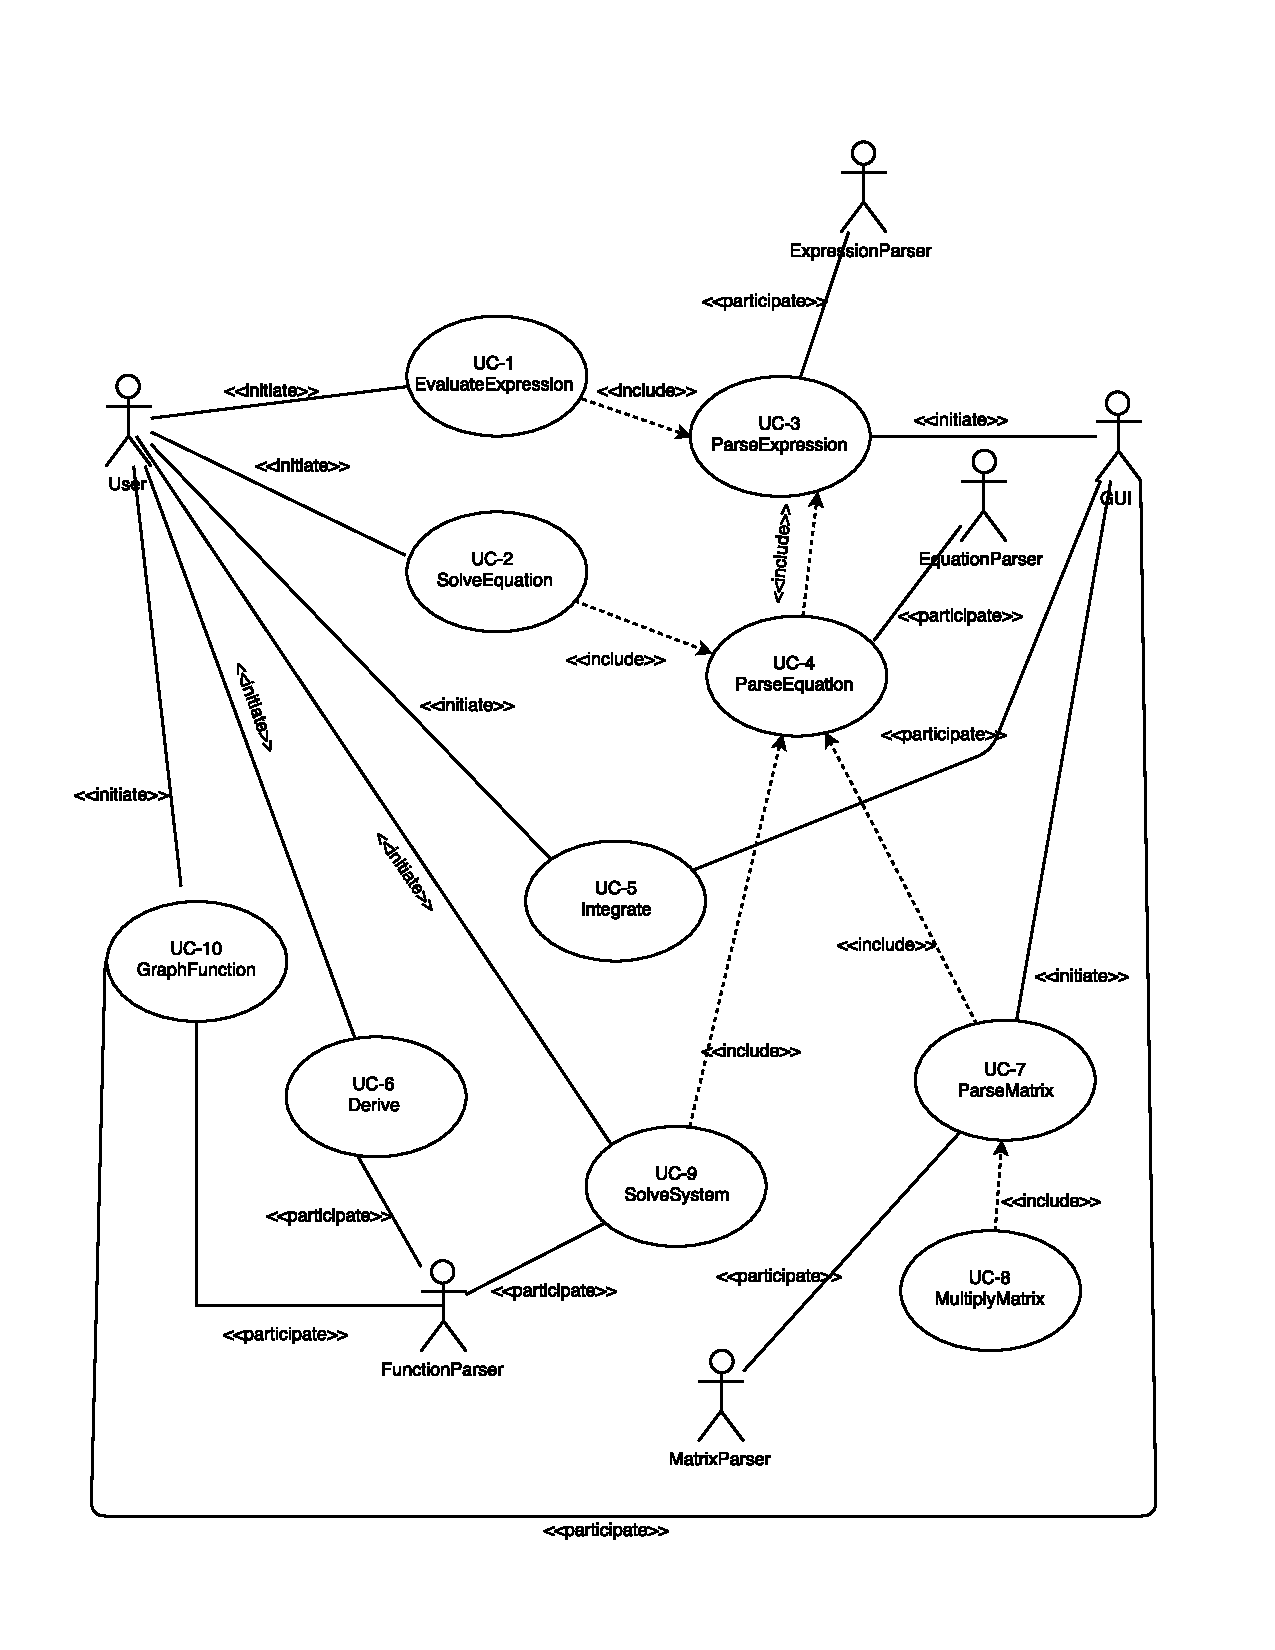
\includepdf[pagecommand={}]{usecasediagram.pdf}

\section{Traceability Matrix}

\begin{center}
\begin{tabular}{|l|l|l|l|l|l|l|l|l|l|l|}
\hline
      & UC-1 & UC-2 & UC-3 & UC-4 & UC-5 & UC-6  \\ \hline
REQ1  & X    &   X   &    &      &      &            \\ \hline
REQ2  & X    &      &      &      &      &            \\ \hline
REQ3  & X    &      &      &      &      &            \\ \hline
REQ4  &      &     &    X  &  X    &      &             \\ \hline
REQ5  &      &     &   X   &  X   &      &             \\ \hline
REQ6  &      &      &      &      &  X   &          \\ \hline
REQ7  &      &      &      &      &     &  X        \\ \hline

\end{tabular}
\end{center}

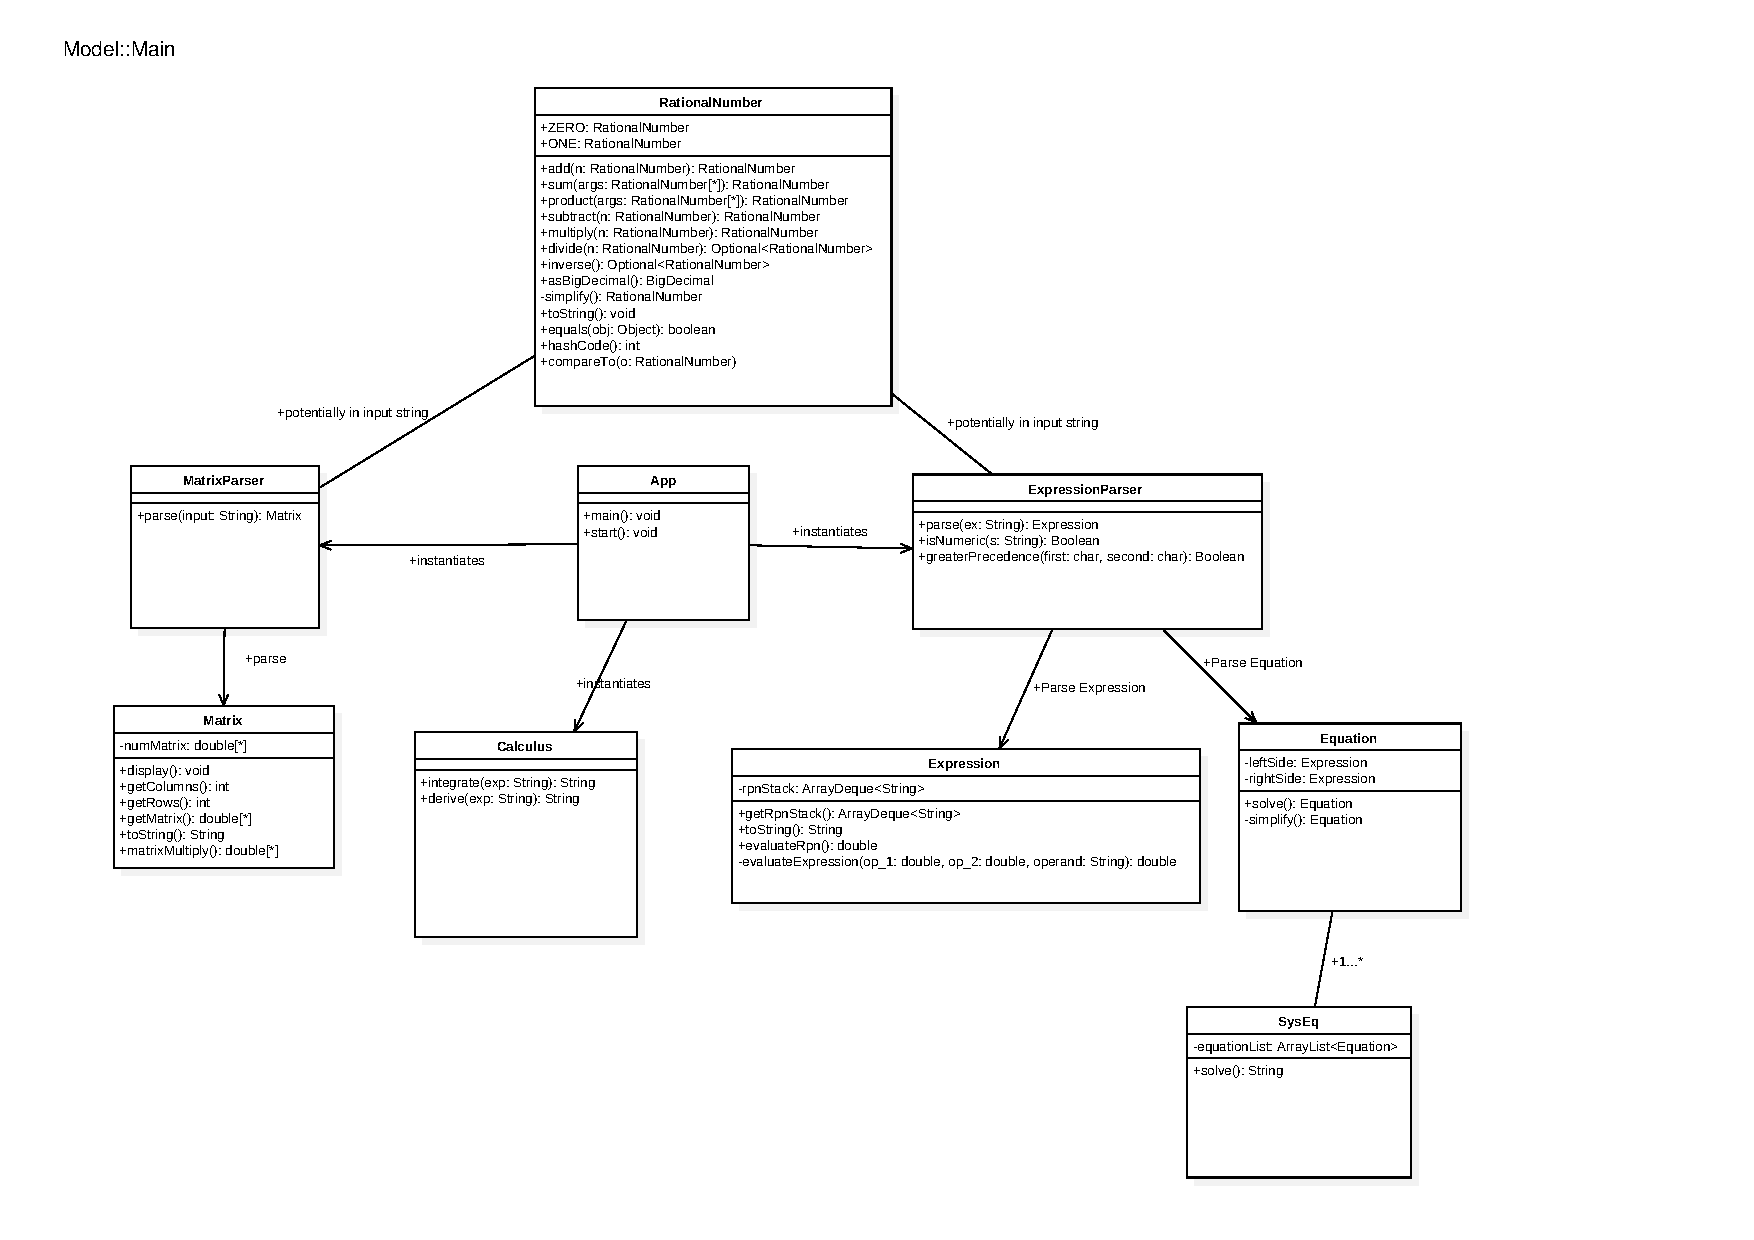
\includepdf[pagecommand={}]{UMLClassDiagram.pdf}
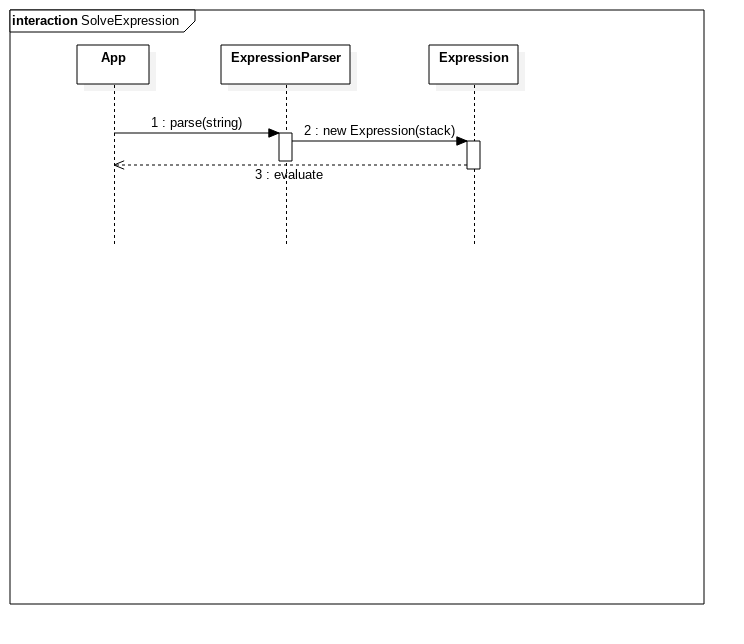
\includepdf[pagecommand={}]{sequencediagrams/sd1.png}
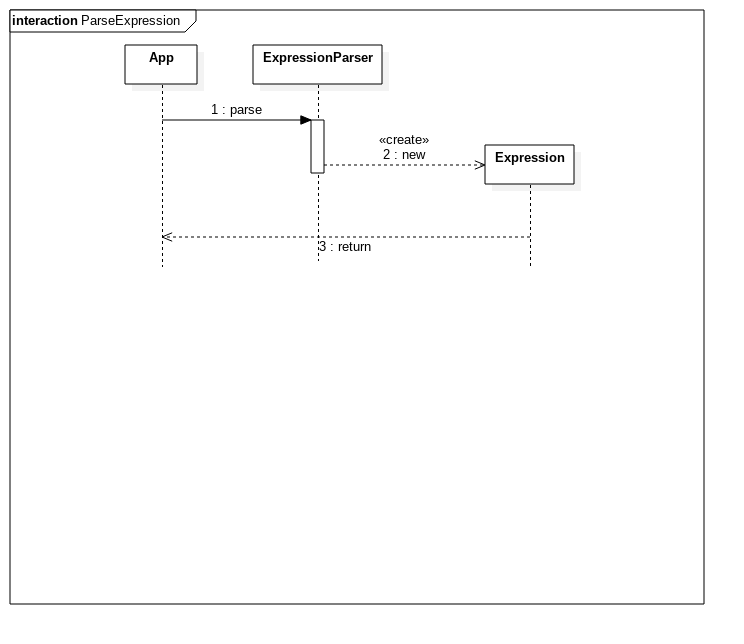
\includepdf[pagecommand={}]{sequencediagrams/sd3.png}
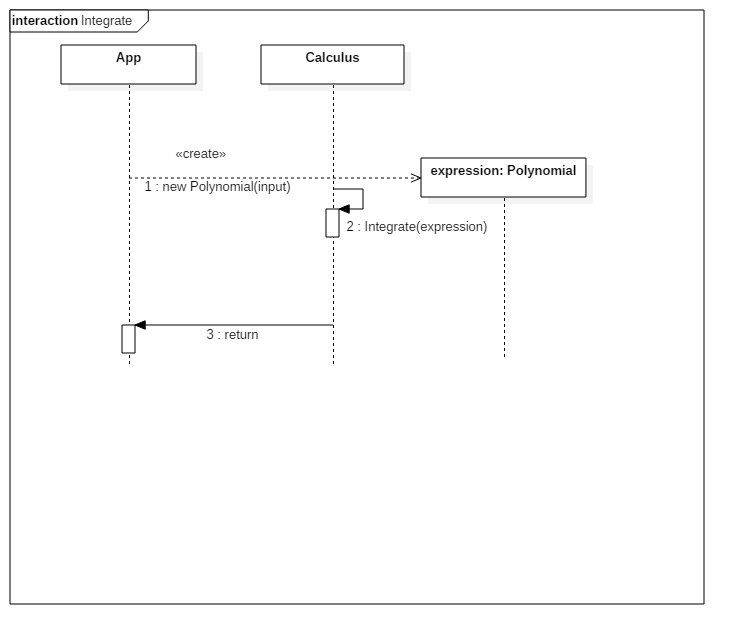
\includepdf[pagecommand={}]{sequencediagrams/sd4.png}
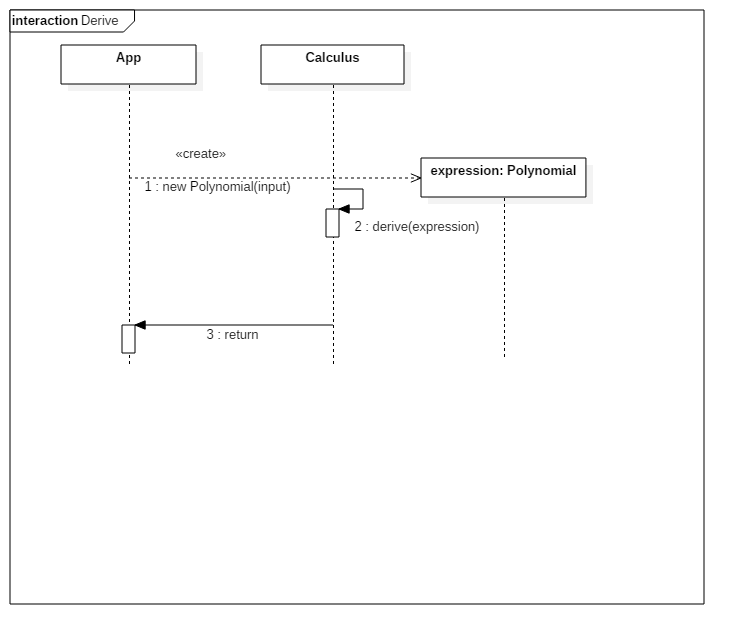
\includepdf[pagecommand={}]{sequencediagrams/sd5.png}
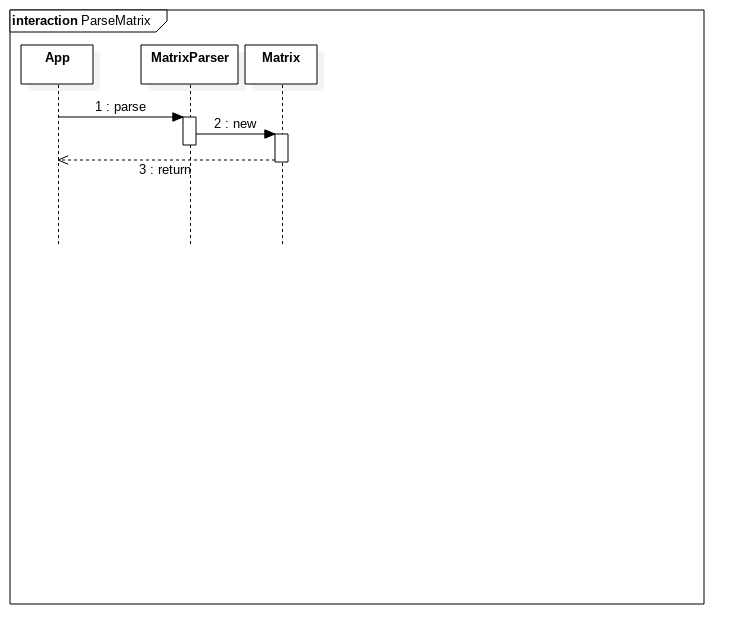
\includepdf[pagecommand={}]{sequencediagrams/sd6.png}
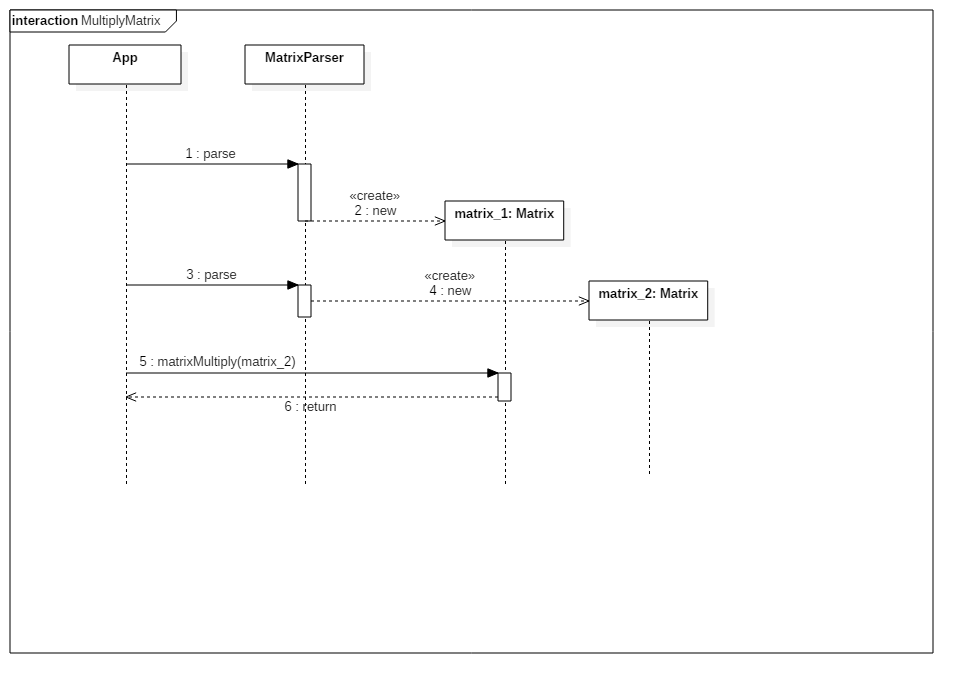
\includepdf[pagecommand={}]{sequencediagrams/sd8.png}


\end{document}
